%% This is stripped of all the AGU- comments, go grab a new copy to submit!

\documentclass[main.tex]{subfiles} %imports preamble and class from main file
%\usepackage{apacite}
%\usepackage{url} %this package should fix any errors with URLs in refs.


%\journalname{Geophysical Research Letters}


\begin{document}

%\title{Enhanced Dehydration Weakening of Antigorite Driven by Slow Shear Heating: Insights from High-Pressure Experiments with a Modified Apparatus Stiffness}


\authors{Eric Burdette and Greg Hirth}

\affiliation{1}{Department of Earth, Environmental and Planetary Sciences, Brown University, Providence, RI, USA}

%\correspondingauthor{Eric Burdette}{eric\_burdette@brown.edu}

\begin{keypoints}
\item Apparatus stiffness was reduced by an order of magnitude with a soft spring added to the loading column.
\item Increased weakening rates during dehydration correlate with both apparatus compliance and imposed load-point displacement rate ($V_0$).
\item High reaction extent and fluid-filled porosity in the center of recovered specimens indicates shear enhanced reaction and resulting weakening. 
\end{keypoints}

\doublespacing

\begin{abstract}
Deformation experiments were conducted to investigate the influence of apparatus stiffness on frictional stability during dehydration of antigorite. These experiments also provided a novel way to constrain relationships between fault slip rate and reaction weakening. Experiments were conducted at a confining pressure of 1 GPa using a Griggs apparatus with a modified loading column. During experiments, the temperature was ramped from 400 to 700°C over 600 seconds, while deformation was imposed with varying load-point displacement rates.  No stick-slip behavior was observed during the experiments, despite an order of magnitude lower apparatus stiffness, suggesting there are inherent differences in the frictional stability between low pressure (where stick-slip is observed during dehydration) and high pressure experiments. Fault slip at high pressure may be stabilized by higher dehydration temperatures and higher shear stresses prior to the onset of dehydration reactions. In comparison to reference experiments conducted with an unmodified stiffness, the weakening rate during dehydration\ increases by a factor of two. In addition, the time (and therefore imposed temperature) at which the maximum weakening rate is observed decreases linearly with increasing maximum weakening rate. Microstructures in the deformed samples illustrate much greater reaction extents (locally $>50\%$) relative to the reference experiments ($<1\%$), with decreasing reaction extent away from the primary slip surfaces.  These observations indicate that the dehydration reaction is enhanced by additional shear dissipation resulting from a tenfold increase in displacement per increment of weakening. The shear-enhanced reaction mechanism could potentially generate runaway slip in subduction zone settings, leading to intermediate-depth earthquakes.\\ 
\\
\\
Plain Language Summary:
The mechanisms that promote intermediate depth earthquakes (50-200km) observed in subduction zones remain poorly understood because brittle materials are generally too strong at low temperature and high pressure to fracture and slide.  Reactions in water-bearing minerals are thought to counteract the influence of high pressure, allowing brittle failure. However, previous studies conducted at mantle pressures only show evidence for stable fault slip that would not produce earthquakes. The experiments presented here show that when we make our high-pressure deformation machine less stiff (resulting in a larger stored energy to drive slip), samples react, and weaken. With the lower apparatus stiffness, pronounced shear heating leads to more rapid (though still stable) stress drops. The shear heating mechanism can be scaled to natural conditions to investigate processes that lead to earthquakes in subduction zones. 

\end{abstract}


%% ------------------------------------------------------------------------ %%
%
%  TEXT
%
%% ------------------------------------------------------------------------ %%


\section{Introduction}

Magnitude 8+ earthquakes occur in subduction zones at depths of 50-100 km where estimated pressures are greater than 1 GPa. At these conditions, below the normal seismogenic zone, most subduction zone materials are extremely strong or deform in a stable rate-strengthening manner, which inhibits earthquake nucleation \citep{Scholz1998}. Thus, these intermediate-depth earthquakes have long been hypothesized to result from dehydration embrittlement of serpentinite \citep{Raleigh1965}, or other hydrous phase, as well as other processes associated with dehydration reactions \citep[c.f.][]{Hacker2003, Rutter2009, Ferrand2017}). However, some experimental studies conducted at mantle pressures indicate stable sliding during dehydration of serpentinite \citep{Chernak2011, Proctor2015, Okazaki2016, Ferrand2017, Gasc2017faulting}.  Here we investigate the possibility that differences in frictional stability during dehydration of antigorite arise from differences in apparatus stiffness. Our new experiments show stable sliding during dehydration, however, we also find evidence for weakening rates enhanced by shear heating. When scaled to natural conditions, such shear heating mechanisms could account for some seismicity.  

Previous experiments on serpentinite show a range of slip behaviors at different confining pressures. For example, nominally drained experiments on antigorite conducted in a gas apparatus at confining pressures below 200 MPa show transitions from distributed shear, to slow slip, and finally to stick-slip behavior as temperature is increased above the dehydration temperature \citep{Okazaki2015}. In contrast, experiments conducted in Griggs-type solid-medium apparatuses at 1-1.5 GPa confining pressure show only slow (stable) slip during dehydration, with no rapid load drops \citep{Proctor2015, Okazaki2016} under both drained and un-drained conditions.  Similarly, experiments conducted at pressures up to 4 GPa in the D-DIA apparatus do not show evidence for stick-slip during dehydration of pure antigorite based on acoustic emission records (Ferrand et al., 2017; Gasc et al., 2017); the acquisition rate of stress measurements in the D-DIA make it difficult to identify stick-slip from mechanical data. These differences make it difficult to extrapolate relationships to conditions appropriate for intermediate earthquakes.  Here we investigate the possibility that this apparent discrepancy between low- and high-pressure experiments can be explained by differences in the apparatus stiffness.

For materials that develop frictional fault surfaces, such as antigorite at our deformation conditions \citep[e.g.][]{Proctor2016}, mechanical behavior is often modeled using rate-and-state friction that describes weakening or strengthening with time and slip velocity. The model has three parameters to describe the evolution of friction: a is the direct logarithmic velocity dependence of the friction coefficient, b and Dc combine to describe displacement and time dependent evolution of friction. (a-b) is positive if steady-state friction is an increasing function of velocity.  Frictional stability criteria (i.e., defining conditions where stable rather than unstable fault slip occur) for materials that obey rate and state friction can be defined using the relationship \citep[e.g.][]{Ruina1983}:
\begin{equation} \label{eq:SH1}
    \frac{K}{\sigma_n}\geq\frac{-(a-b)}{D_c},
\end{equation}

where K is shear stiffness (the elastic relationship between shear stress and shear displacement on the fault surface), and $\sigma_n$ is normal stress. Three responses to velocity perturbations are possible, depending on the velocity-dependence of friction. For velocity strengthening (a-b) > 0, the system is stable. For velocity weakening, the system is conditionally stable if equation (\ref{eq:SH1}) is satisfied, but the system is intrinsically unstable if $\frac{K}{\sigma_n} < \frac{-(a - b)}{D_c}$. The transitions in slip behavior observed by \citet{Okazaki2015} were hypothesized to result from changes in the frictional properties with increasing temperature. 
Equation (\ref{eq:SH1}) shows that increasing K (or, $K/\sigma_n$) promotes stable sliding. Thus, assuming that the frictional properties remain the same at high pressure, one explanation for the lack of stick-slip in the Griggs and D-DIA experiments is that the ratio $\frac{K}{\sigma_n}$ is much larger for the higher confining pressure experiments (Figure \ref{fig:F1}). Alternatively, the frictional behavior might change as a function of confining pressure at a given temperature and strain rate. \citet{Okazaki2015} report an apparatus stiffness of 58 MPa/mm, while the higher pressure apparatus have a stiffness of ~2 GPa/mm (Griggs-type apparatus) and ~200 GPa/mm (D-DIA; see calculation in the appendix), respectively. As described in the next sections, we tested these hypotheses by modifying the stiffness of the Griggs apparatus to match the ratio $\frac{K}{\sigma_n}$ (and thus stability) of \citet{Okazaki2015}, while running experiments using the same procedures as \citet{Proctor2015}.

\begin{figure}[p]
  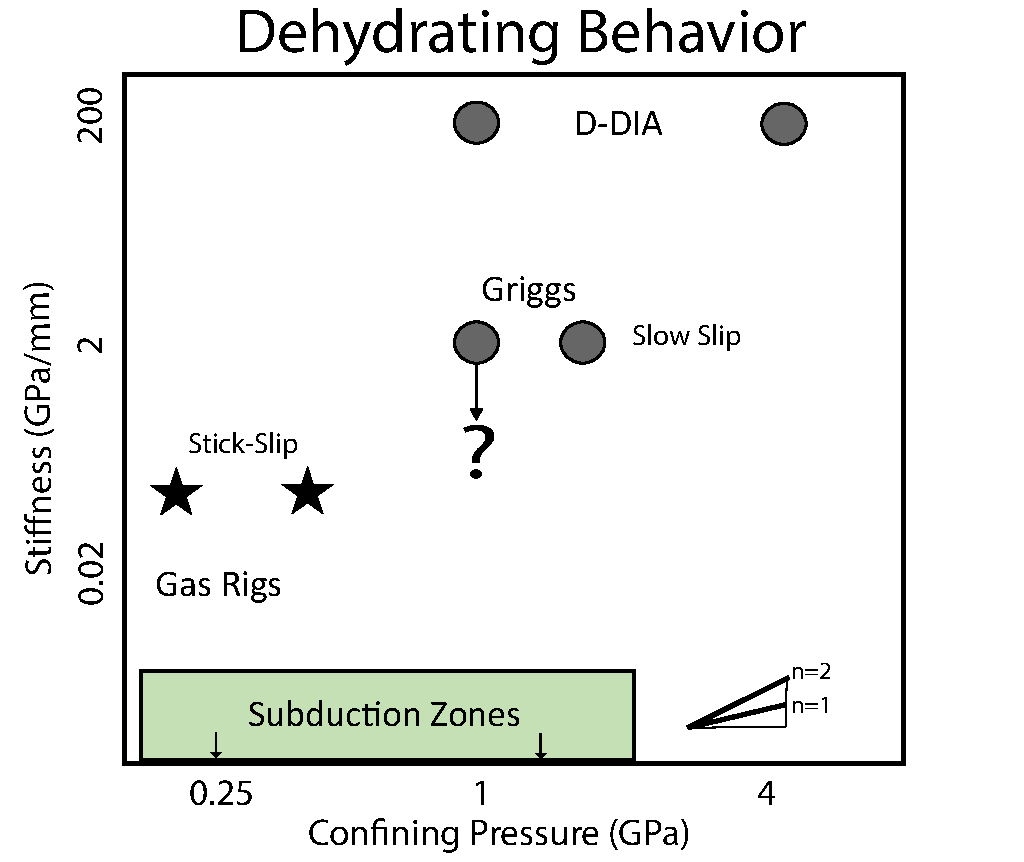
\includegraphics[width=\textwidth]{Figures/F1.pdf}
  \caption[Apparatus stiffness vs. pressure for antigorite deformation studies]{Confining pressure and corresponding apparatus stiffness plotted for conditions of previous experimental studies of mechanical behavior during dehydration of antigorite. D-DIA studies referenced are those of \citet{Hilairet2007, Ferrand2017, Gasc2011}.  Griggs studies referenced are those of Chernak et al. (2011), Proctor et al. (2015), and Okazaki et al (2016). Gas apparatus experiments referenced are those of Okazaki et al. (2015), and Murrell et al. (1976). Plotted on a log scale to illustrate stiffness ($< 5*10^{-5}$ MPa/mm, methods of Fletcher and McGarr 2006) and pressure in subduction zones.}
  \label{fig:F1}
\end{figure}

The modification of the apparatus also allowed us to explore the role of shear dissipation in reaction weakening. As frictional slip proceeds during dehydration of antigorite at 1 GPa confining pressure, pore fluid pressure increases due to a reaction producing forsterite, enstatite/talc, and water causing samples to weaken in response to decreasing effective normal stress. Temperature ramping results in a bell-shaped reaction rate versus time curve, with a peak at a characteristic reaction extent (\cite{Vyazovkin2011, Trittschack2014}; Trittschack et al., 2014 illustrate this behavior for brucite and serpentine). \citet{Chernak2011} illustrate that the weakening rate during dehydration increases with increasing temperature ramp rate (indicting a relationship between reaction rate and weakening rate). \citet{Proctor2015} illustrate that the weakening arises from an increase in pore-fluid pressure by comparing drained (reaction with no pore fluid pressure) and the undrained dehydration experiments, consistent with the related work of and \citet{Murrell1976}. 
The reduction in strength during pore-fluid weakening is accompanied by an elastic response of the machine. The system can be described by a simple slider-block model with equations:
\begin{equation} \label{eq:SH2}
    \tau=\mu\left(V\right)\ast\left(\sigma_n-P_f(\omega)\right),
\end{equation}
\begin{equation} \label{eq:SH3}
    V\ =\frac{1}{K}\left(-\frac{d\tau}{dt}\right)+V_0,
\end{equation}

Where $\tau$ is shear stress, V is slip velocity, $\mu$ is the velocity-dependent friction coefficient, $P_f$ is pore fluid pressure as a function of reaction, $\omega$ is reaction extent, and K is shear stiffness. As shown by equations (\ref{eq:SH2}) and (\ref{eq:SH3}), the friction coefficient is connected to an elastic response through its dependence on velocity. Pore fluid pressure can be affected by the elastic response through shear dissipation (a function of velocity V) that drives increased reaction rates.  Similar to the rate-state friction criteria in equation (\ref{eq:SH1}), the inclusion of shear heating results in more complex conditional stability criteria that depend on a minimum stiffness, starting shear stress, thermal diffusivity, and permeability (examined by \citet{Brantut2012}). In the experiments described here, we reduced K by a factor of ten, which leads to a tenfold increase in shear dissipation that can enhance reaction and be assessed through the time evolution of strength.


\section{Materials and Methods}

    \subsection{Materials and Sample Preparation}
        Antigorite samples were synthesized from a serpentinite collected from the Nagasaki metamorphic belt in Japan; this sample is predominantly antigorite (98\%) with minor diopside, spinel and magnetite. The serpentinite was crushed and sieved to prepare gouge samples with a grain size of 20 um to 45 um. Powder was washed and magnetically separated following sieving. The weight of gouge sample used for each run was 150.0 mg, resulting in a sample thickness of 1.1 mm without any optically visible porosity ($<1\%$) after hot-pressing for 12 hours at 400°C and 1 GPa confining pressure.
        
    \subsection{Deformation Procedure and Sample Assembly}
        Experiments were conducted in a Griggs-type triaxial press \citep{tullis1986experimental} using NaCl as a confining medium, at a confining pressure of 1 GPa and a temperature range from 400 to 700°C. Samples were deformed at imposed displacement rates ($V_0$) of 0.18, 0.36, or 1.8 $\mu$m/s using an AC motor. We refer to $V_0$ as the load-point displacement rate; specifically, $V_0$ is the displacement rate measured between the top of the load cell and the upper platen (Figure \ref{fig:F2}). 
        
        \begin{figure}
          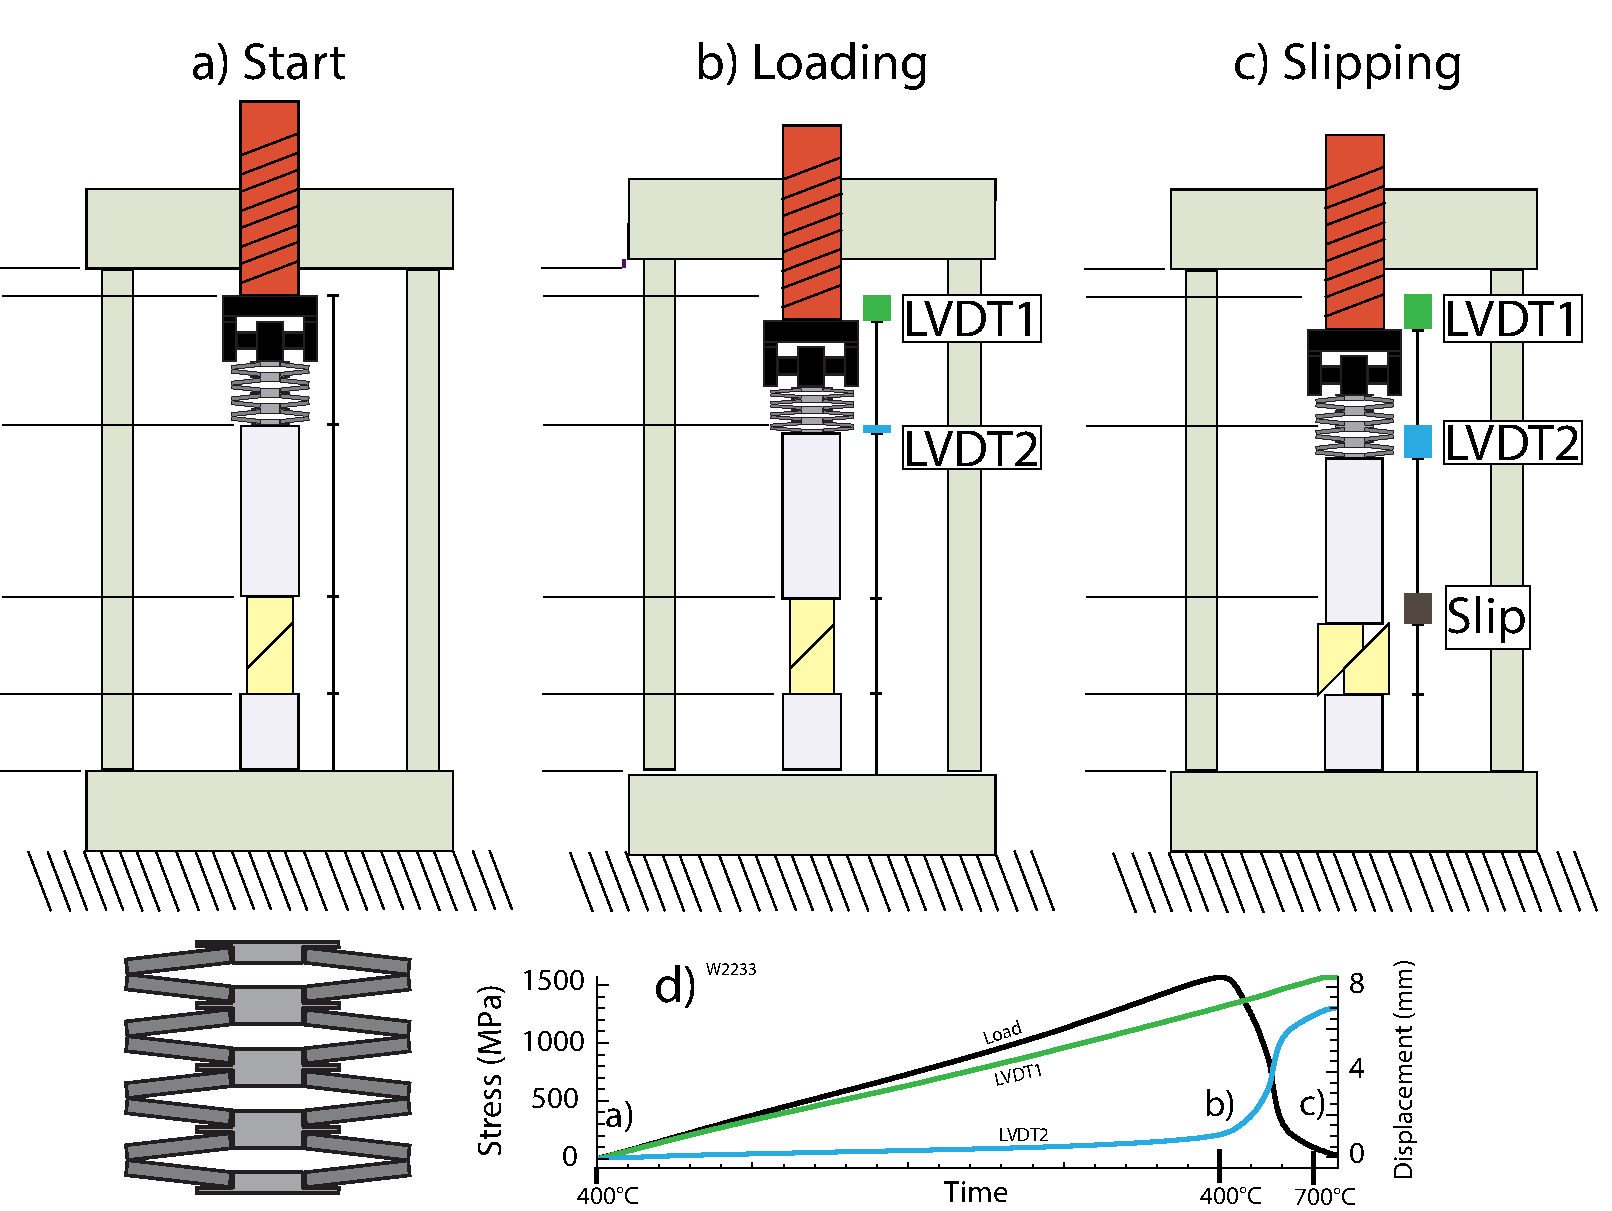
\includegraphics[width=\textwidth]{Figures/F2.pdf}
          \caption[Schematic of compliant spring and apparatus movement during deformation/dehydration]{Schematic figure illustrating relative movement of modified triaxial apparatus elements during antigorite deformation/dehydration runs (W2333 is depicted). (a) Initial apparatus position with no differential stress applied to the gouge sample. (b) Sample loaded to peak stress. Axial loading is applied by a ball screw represented by the cross-hatched element at the top of the column. Elastic displacement is stored primarily in the disk springs with a small portion stored in the column below the disk spring. (c) Apparatus position during and after weakening.  Note that the majority of displacement is generated by the spring elements. (d) Time history of the load and displacement for both transducers (LVDT1\&2). Black bars indicate start of the temperature ramp at 400°C, and the end of temperature ramp at 700°C.}
          \label{fig:F2}
        \end{figure}
        
        Powder was placed between alumina shear pistons cut at angles of 30, 45, or 60 degrees to the axial stress and placed inside a cylindrical Ag jacket with wall thickness of 0.25 mm. Ag disks were placed at the end of each shear piston and mechanically sealed during a short cold pressing step. Sample temperature was measured using a Pt–Pt10\%Rh thermocouple placed next to the jacket at the sample center (Figure \ref{fig:F3}b). Samples were brought to 1 GPa and 400°C, allowed to equilibrate for 12 hours, and then loaded at a constant load-point displacement rate. After reaching peak stress and the initial onset of weakening (Figure \ref{fig:F3}), the temperature setpoint was ramped from 400-700°C at 0.5°C/s while $V_0$ was maintained (calculations indicate <1°C sample temperature lag, see supporting information). After reaching 700°C, all samples were first quenched under load to 300°C in ∼1 min and then returned to ambient conditions over 1–2 h. Samples were then impregnated with epoxy, cut and polished into thin-sections for microstructural analysis.
        \begin{figure}
          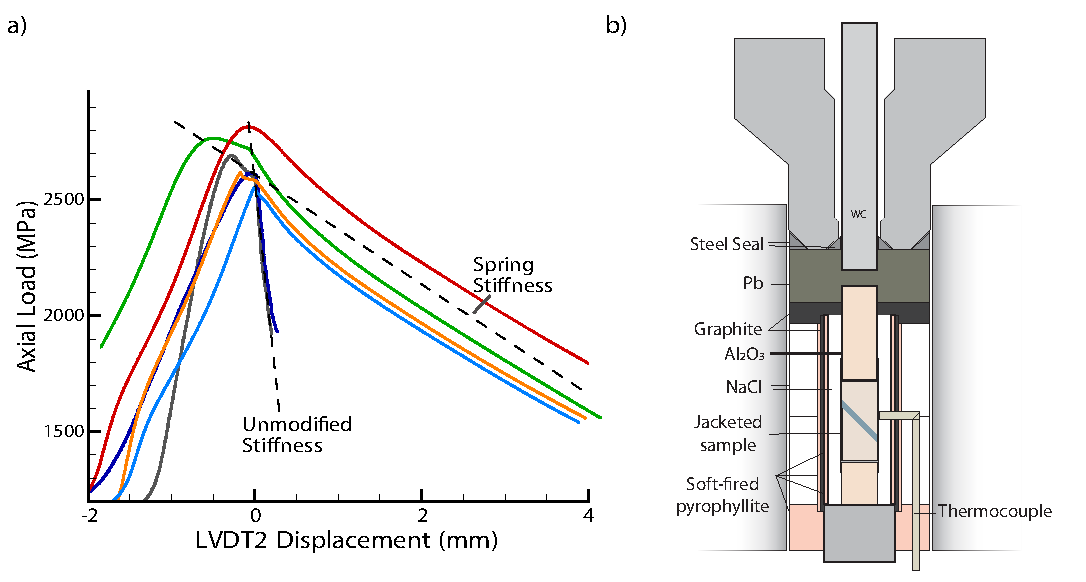
\includegraphics[width=\textwidth]{Figures/F3.pdf}
          \caption[Load-displacement plot and gouge sample assembly]{Figures summarizing recorded axial load vs LVDT2 displacement and a depiction of the sample assembly. (a) Load plotted against displacement for dehydration runs, with displacement referenced to the recorded value at initiation of the temperature ramp. Dashed reference lines are plotted for the static stiffness of the standard and modified apparatus. (b) Schematic illustration of the experimental apparatus inside the pressure vessel. Sample powder is contained between two sawcut alumina shear pistons inside the silver jacket.}
          \label{fig:F3}
        \end{figure}
    
    \subsection{Deformation Apparatus}
        The loading frame of the press was modified to change stiffness between experiments by inserting a modular column comprised of paired Belleville disk springs.  The original load cell was replaced with a smaller load cell to accommodate this change. The unmodified apparatus axial stiffness ($K_{Apparatus}$) is 1.97 GPa/mm. The modified apparatus is an order of magnitude less stiff (0.194 GPa/mm) with the addition of 4 pairs of Belleville disk springs. This modification of stiffness leads to an order of magnitude more sample displacement for a given decrease in stress. These stiffness values include the tie-bar elements of the load frame and the ball screw used to drive the loading column (see supporting information). For comparison, the gas confining media apparatus used by \citet{Okazaki2015} is less stiff than our modified apparatus. Thus, we can conduct experiments at similar values of $\frac{K}{\sigma_n}$ (i.e. equation \ref{eq:SH1}) as those conducted by \citet{Okazaki2015} ; (i.e., (155 MPa/mm)/(~200 MPa) = 0.78/mm for the gas apparatus used \citep{Okazaki2015}, and (194 MPa/mm)/(~1000 MPa) = 0.19 GPa/mm for our modified apparatus).
        
        In the triaxial apparatus shear and normal stress evolve together (see supporting information). At constant pressure, they both evolve as a function of axial stress $\sigma_1$. For simplicity, we report measured quantities axial stress, LVDT2 displacement, and axial stiffness $K_{Apparatus}$ instead of the derived shear quantities. An additional LVDT (referred to as LVDT2 in Figure \ref{fig:F2}) was added below the springs to provide a better measurement of sample displacement ($V_{sample}$). To present the data in the most straightforward way, in the figures we plot measured values of displacement from LVDT2. In detail, the slopes on these curves show are somewhat greater stiffness because they reflect $K_{Upper\ Column}$ and not $K_{Apparatus}$ (Figure \ref{fig:S1}). Plotting the raw data in this way has no effect on our conclusions.

        
    \subsection{Data Recording and Treatment}
        Mechanical data were recorded at 1kHz, then anti-alias filtered and reduced for storage.  Precision in load and pressure is 0.1 MPa, while precision in displacement is 0.1 \(\mu\)m. Recorded load and displacement data were converted to shear stress and shear displacement using methods outlined in the data reduction program RIG 1.3 by Matej Pec.

\section{Results}

    \subsection{Mechanical Results}
        Load versus displacement curves for temperature-ramping experiments (all with a temperature ramp rate of 0.5°C/s) are illustrated in Figure \ref{fig:F3}a. Here we report axial load in MPa by dividing the axial force by the area of the 1/4 inch diameter loading piston. The slopes of the load versus displacement curves for experiments conducted using the unmodified loading column approach, but remain less than, the apparatus stiffness. Similarly, the slope of the load versus displacement curves during weakening for experiments conducted with the modified loading column plot near the modified apparatus stiffness (Figure \ref{fig:F3}a and Figure S2). Calibration experiments (shown in the  supporting information) indicate that the higher initial slopes during weakening arise from frictional hysteresis between surfaces of the Belleville springs, and thus the load versus displacement curves in Figure \ref{fig:F3} also reflect weakening with a slope similar to the machine stiffness.  
        
        Even with the significant decrease in apparatus stiffness, the samples unload stably in all experiments. We do not observe stick-slip. We can compare details of the weakening using characteristics outlined in \cite{Proctor2015}. Plots of displacement rate and weakening rate (d$\sigma_1$/dt) versus time exhibit two peaks during the temperature ramps in both modified-stiffness (Figure \ref{fig:F4}a) and unmodified-stiffness experiments. The first peak initiates just after the onset of the imposed temperature increase (Figure \ref{fig:F4}a, the first peak overlaps with second peak for W2233); previous studies show that this weakening occurs in a similar way under both drained and undrained pore fluid pressure conditions \citep{Proctor2015}, and is interpreted to reflect the effect of temperature on the strength of antigorite. The second peak follows 100-500 seconds later with a higher d$\sigma_1$/dt, and proceeds until the sample weakens to the final strength. The second event is driven by pore fluid produced by the dehydration reaction \citep[e.g.][as outlined in introduction]{Proctor2015}. The time after the ramp initiation (the x axis in Figure \ref{fig:F4}a) where the 2nd peak in d$\sigma_1$/dt is observed is a proxy for the time required to achieve a characteristic reaction extent. The magnitude of the maximum weakening rate (d$\sigma_1$/dt) is a proxy for reaction rate. In the discussion section, we distinguish these concepts from complications arising from rate-dependent friction. 
        \begin{figure}
          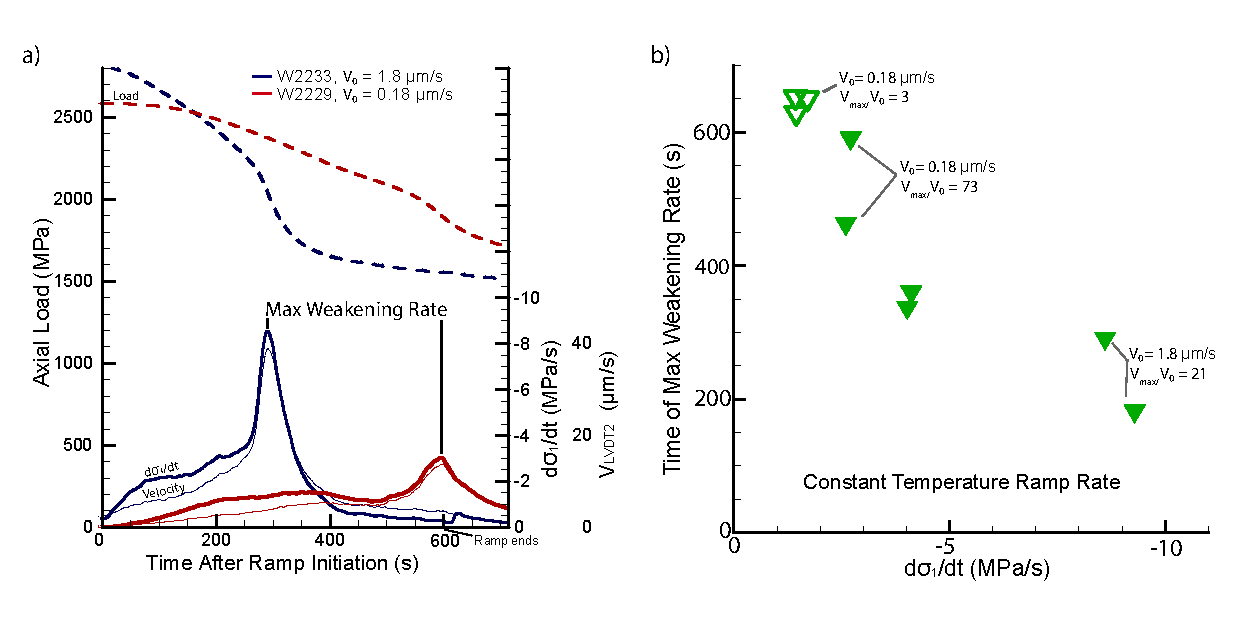
\includegraphics[width=\textwidth]{Figures/F4.pdf}
          \caption[Plots showing mechanical data derivatives during dehydration and times of their maxima by experiment]{(a) Time history of recorded load, velocity, and weakening rate during dehydration. Run conditions are noted in the plot. b) Observed time (after temperature ramp start) of the maximum weakening rate plotted against the magnitude of the maximum weakening rate; the load-point displacement rate ($V_0$) and $V_{max}$/$V_0$ are noted near data points. Open triangles are experiments with the unmodified stiffness, solid triangles are modified-stiffness experiments.}
          \label{fig:F4}
        \end{figure}
        
        While unstable slip is not observed, experiments conducted with the modified stiffness exhibit higher maximum fault displacement rates and a decrease in the time at which the maximum weakening rate occurs. Peak sample displacement rates are 20 to 100 times greater than the imposed displacement rate ($V_0$) for intervals of 10s of seconds (Figure \ref{fig:F4}a). The time of the maximum  d$\sigma_1$/dt is plotted against the magnitude of the maximum  d$\sigma_1$/dt in Figure \ref{fig:F4}b. The experiments with modified stiffness exhibit slightly larger weakening rates and much higher sample displacement rates. In addition, experiments conducted with higher $V_0$ achieve maximum sample displacement rates 50 and 450 seconds earlier than observed in experiments with unmodified stiffness deformed at the same conditions (Figure \ref{fig:F4}b). Because all of the temperature ramps start at 400°C with the same temperature ramp rate, the shorter time required to achieve the peak slip rate correlates with imposed temperatures that are 25 to 225°C lower.
        
        The maximum weakening rate in our modified-stiffness experiments also increases with an increase in $V_0$ (Figure \ref{fig:F7}). The weakening rate (d$\sigma_1$/dt) increases by a factor of 3 for a factor of 10 change in $V_0$. Figure \ref{fig:F7} illustrates that the maximum weakening rate also correlates with the magnitude of differential stress at the onset of the temperature ramp. 
        \begin{figure}
          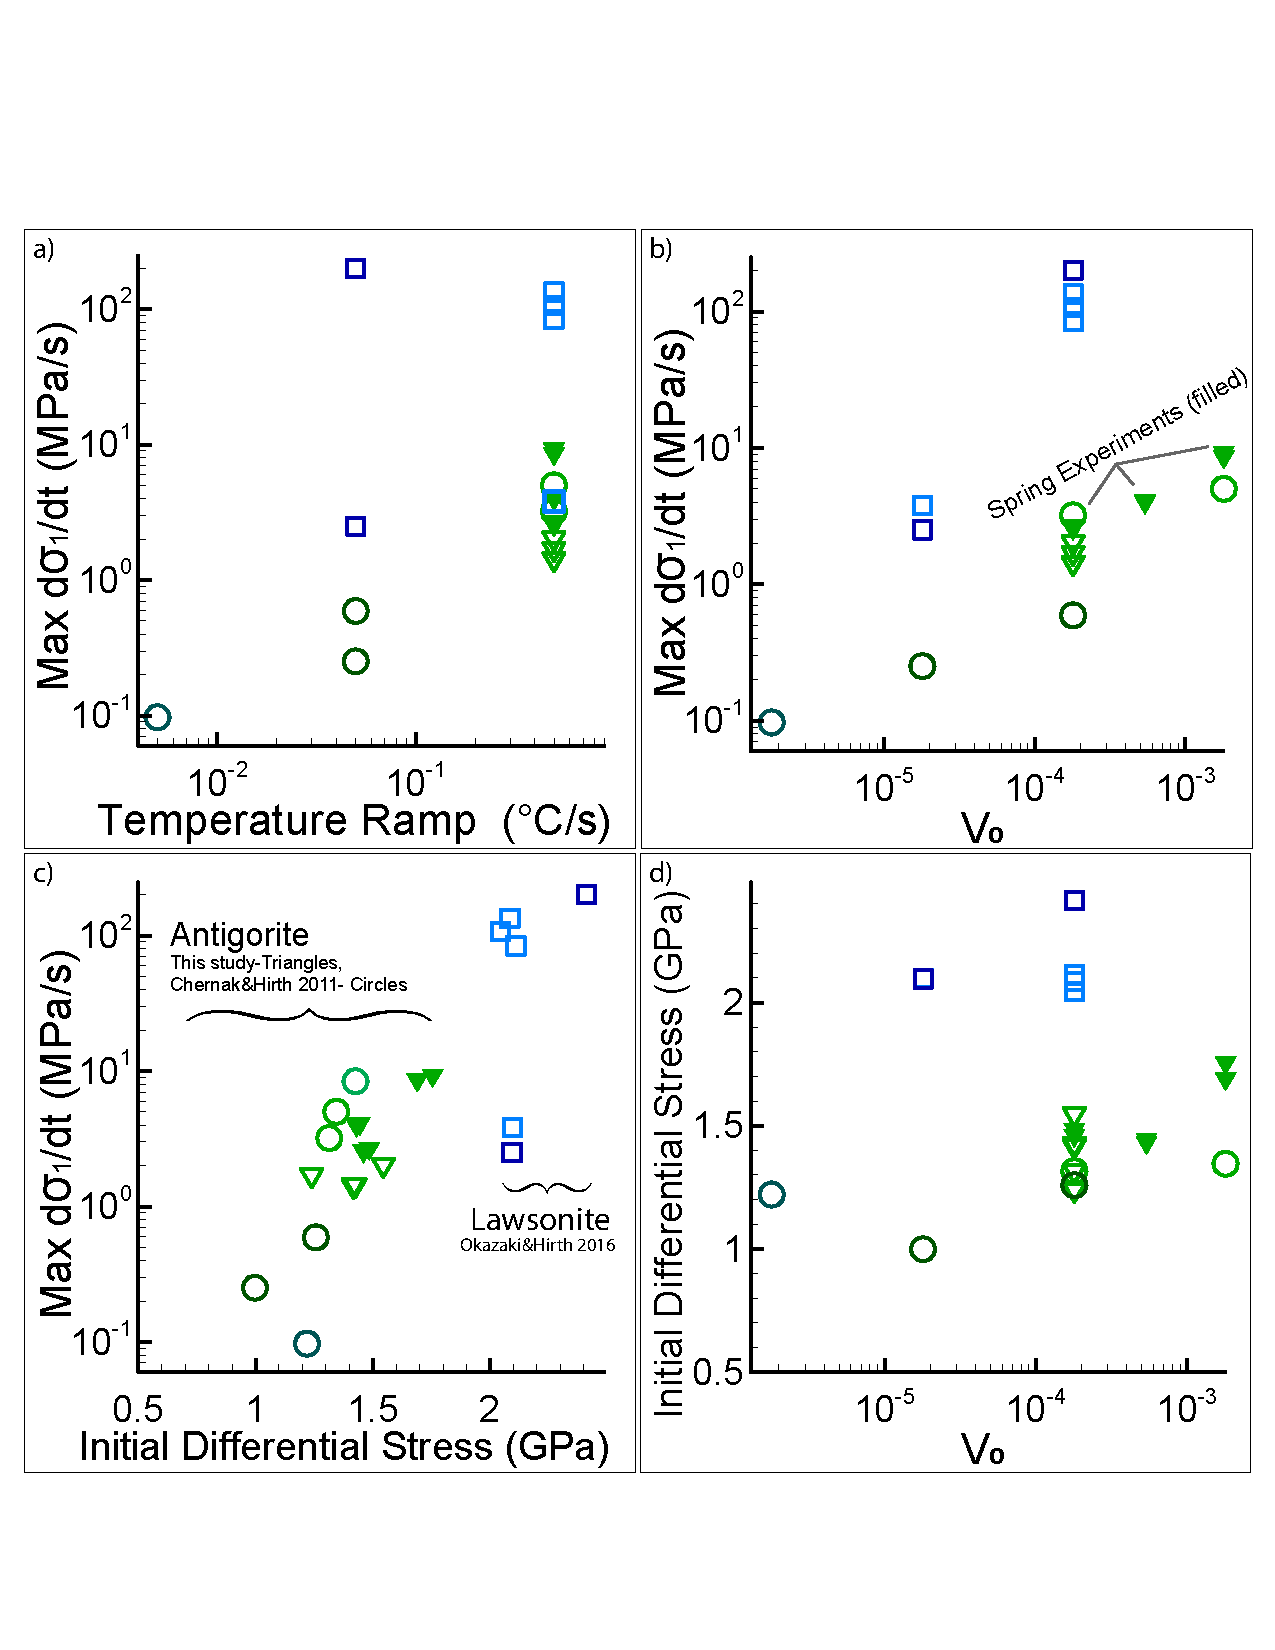
\includegraphics[width=\textwidth]{Figures/F7.pdf}
          \caption[Summary of characteristic variables during dehydration of lawsonite and antigorite]{Open symbols are runs with unmodified stiffness. Circles are Antigorite data from Cernak and Hirth 2011, squares are Lawsonite data from Okazaki and Hirth 2016 for comparison, and triangles are this study. Darker shades of color for each materials denote a lower ramp rate. (a) Plot of maximum weakening rate vs. temperature ramp rate. (b) Plot of maximum weakening rate vs. imposed load-point displacement. (c) Plot of weakening vs. differential stress at the initiation of temperature ramping. (d) Plot of initial differential stress vs. imposed load-point displacement rate.}
          \label{fig:F7}
        \end{figure}
    
    \subsection{Microstructural Observations}
        Microstructural analyses of our samples illustrate evidence of dehydration reactions occurring in the deformed samples. SEM micrographs of the sample with the largest observed weakening velocity (W2233, $V_0 = 1.8 \mu$m/s) and a hydrostatically annealed sample that experienced the same imposed temperature-pressure protocol are illustrated in Figure \ref{fig:F5}. The deformed sample exhibits spatial variations in forsterite content, indicating variations in reaction extent. The highest reaction extent is observed in the center of the sample adjacent to the high-displacement faults. A high reaction extent inside the fault zone is illustrated by a large fraction of forsterite (33\% by area) and porosity (12\% by area) in the quenched sample (Figure \ref{fig:F5}). 200 $\mu$m outside of the fault zone, the reaction extent is significantly lower (83\% unreacted antigorite, 15\% forsterite, and 2\% porosity, all by area). The forsterite grains are rounded and <2 $\mu$m in diameter, often in bands oriented parallel to the fault zone. Outside of the primary fault zone forsterite grains with similar diameter form but are concentrated in pores between grains. Similar microstructures, but with smaller reaction extents, are shown for samples deformed with lower $V_0$ (W2230, $V_0$ = 0.54 μm/s; W2229, $V_0$ = 0.18 $\mu$m/s (Figure \ref{fig:F6}). All of these samples illustrate significantly greater reaction extent than that observed in samples of antigorite deformed with the unmodified stiffness using the same temperature ramp protocol (e.g., sample W1892 from \citet{Proctor2015}).
        \begin{figure}
          \includegraphics[width=\textwidth]{Figures/F5.pdf}
          \caption{Images of a deformed sample containing high forsterite (Fo) content (a proxy for reaction extent visible in electron imaging) and porosity that decreases away from fault surfaces, as well as a reference hydrostatic sample conducted with the same temperature protocol with no visible reaction products. Noted fractions are area percent.}
          \label{fig:F5}
        \end{figure}
        
        \begin{figure}
          \includegraphics[width=\textwidth]{Figures/F6.pdf}
          \caption[Temperature rise and corresponding recovered microstructure]{Plotted: Predicted temperature rise above imposed (ramping) temperature as a function of time calculated from supporting information equation \ref{eq:S1}. The highest temperature and reaction extent occur in experiment W2233-0.2-4 which is featured in Figure \ref{fig:F4}a. Images: Recovered fault surface microstructure of several samples where reacted forsterite content (Fo) is highlighted: W2230, W2229, W2319-I, and W2375-I (clockwise).}
          \label{fig:F6}
        \end{figure}
        
        To investigate microstructures associated with the onset of reaction weakening, some experiments (all with 45° pistons at $V_0$ =1.8 μm/s) were quenched before the imposed temperature reached 700°C.  These samples show the development of localized shear zones along fractures oriented in the R1/Reidel shear orientation. The sample quenched after the smallest amount of displacement shows localized deformation and no evidence for reaction (Figure \ref{fig:F6} W2319-I, quenched at 500°C).  While more difficult to resolve relative to the higher displacement samples, small amounts of reaction products are observed in the gouge zone of the fault that formed in the sample quenched at the onset of weakening (Figure \ref{fig:F6} W2375-I, quenched at 600°C). In contrast, a hydrostatically annealed sample (W-2329-H) that was quenched at 600°C after the same imposed temperature-pressure protocol as W2375-I shows no reaction products (Figure \ref{fig:F5}). In addition, there is minimal evidence for crushing or alignment of the antigorite grains in the hydrostatic sample.
        
        
        The samples deformed with the modified stiffness experience large fault displacement – a direct result of the difference in stiffness. The highest reaction extents are observed within the center of the samples along the fault zones. The outer edges of the samples exhibit much lower reaction extents, indicating that the reaction extent is not a reflection of translation of the sample closer to the graphite furnace. 


\section{Discussion}
    Even with the reduced apparatus stiffness, we do not observe stick-slip events which would be expected if the dehydrating antigorite gouge obeyed rate-and-state friction and was velocity-weakening (given the observations from \citet{Okazaki2015}). Based on comparison with these lower pressure experiments, our observations indicate that the frictional behavior of antigorite changes at high confining pressure for a given temperature and strain rate. Such a transition may arise owing to the activation of rate-strengthening deformation processes, in response to both the higher stresses required for deformation and higher temperatures due to a positive Clapeyron slope of the dehydration reaction up to 1 GPa confining pressure. Consistent with these interpretations, at the conditions of our experiments, rate-strengthening deformation has been reported for antigorite gouge, both within its stability field \citep{Proctor2016} and during dehydration \citep{Chernak2011}.
    
    While we do not observe stick-slip, our results highlight positive feedbacks between slip velocity and reaction weakening rate that are enhanced in the experiments conducted with the modified stiffness. In the following sections we discuss how these observations that indicate these feedbacks arise from shear heating.

    \subsection{Effects of Temperature Ramp Rate, Imposed Velocity on Weakening of Antigorite and Lawsonite}
    In contrast to our observations for antigorite, \cite{Okazaki2016} found that dehydration reactions in lawsonite generate stick-slip events. As outlined below, comparing observations for these materials suggests that the contrasting behaviors during dehydration arise from the differences in the rate-dependence of friction of the reacting materials.
    
    First, the maximum weakening rate in antigorite correlates strongly with temperature ramp rate (Figure \ref{fig:F7}a). This observation indicates that weakening rate in antigorite is controlled by reaction rate that leads to continual pore fluid pressure generation during temperature ramping \citep{Proctor2015}. We repeated unmodified-stiffness experiments on antigorite (open triangles) and reproduce trends from previous work. In contrast, no clear trend in shown for lawsonite in Figure \ref{fig:F7}a, indicating an apparent decoupling between weakening rate and reaction rate. 
    
    Second, for a given temperature ramp rate, the weakening rate increases with $V_0$ for both antigorite and lawsonite, with the effect more prominent for lawsonite (Figure \ref{fig:F7}b). The initial differential stress (i.e., before temperature ramping) increases with $V_0$ for antigorite (Figure \ref{fig:F7}d). In contrast, $V_0$ appears to have little influence on the differential stresses before temperature ramping for lawsonite, although the stresses are approximately two times greater than those for antigorite (Figure \ref{fig:F7}c). From these observations, we conclude that the weakening process for lawsonite (which leads to unstable stress drops) must involve rate-insensitive or weakening friction, in conjunction with critical stability conditions (i.e., equation \ref{eq:SH1}) that are close to our starting conditions (as concluded by Okazaki and Hirth, 2016). In contrast, the velocity strengthening nature of the antigorite friction appears to inhibit instability.
    
    Third, the relationships shown in Figures 7b and 7c for antigorite indicate dissipative processes lead to faster reaction rates – and faster, but apparently stable weakening. In the next section we discuss the roles of rate-dependent friction and pore-fluid weakening on the rate sensitivity of slip during dehydration.

    \subsection{Rate Sensitivity of friction during Pore-fluid Driven Weakening}
        Closer inspection of our data reveals evidence for a rate-weakening effect associated with reaction (likely shear heating). To illustrate this behavior, we outline the expected effects of reaction weakening and stiffness on sample strength and slip velocity using a frictional slider-block model. Equation (\ref{eq:SH2}) can be applied to our tri-axial experiments (for which axial load and axial displacement are measured) using standard linear relationships that account for the angle of the fault zone. At the same conditions as our experiments, \citet{Proctor2015} establish that equation (\ref{eq:SH2}) describes the evolution of strength during dehydration by comparing drained ($P_f=0$), partially drained, and undrained (i.e., sealed) experiments.
        
        \begin{figure}
          \includegraphics[width=\textwidth]{Figures/F8.pdf}
          \caption[Simplified model of changes in mechanical response during dehydration when stiffness is changed]{Schematic plots of stress and slip velocity for a block slider with strength evolution controlled by the change in pore fluid pressure during dehydration (equation \ref{eq:SH2}). (a) Velocity response of an unmodified reference case R, and the predicted response of a rate insensitive system where K is changed. Velocity response is directly proportional to the ratio between standard and modified compliance (1/K) by equation (\ref{eq:SH2}) (b) Expected response of a velocity strengthening material to pore-fluid driven weakening. Rate strengthening is enhanced by extra displacement released during weakening serving to “hold-back” (delay) the weakening velocity and magnitude. This behavior is not observed in our experiments. (c) Expected response of a velocity weakening material to pore fluid driven weakening. Increased velocity enhances weakening, causing peak weakening rate to happen earlier. Reaction rate is also modified to match weakening mechanism of microstructural observations.}
          \label{fig:F8}
        \end{figure}

        The influence of slip velocity on weakening rate during dehydration can be evaluated by comparing experimental data to the result expected for a reference scenario where (a) frictional resistance is assumed to be rate-independent and (b) d$\tau$/dt is fixed by the change in pore fluid pressure resulting from the dehydration reaction driven by the imposed temperature ramp. With this scenario, d$\tau$/dt (and thus d$\sigma_1$/dt) would not be affected by the change in apparatus stiffness (K), and K would govern the relationship between changes in force and changes in displacement (eq. 3). If $V_0$ is much less than the sample slip velocity (as observed in our experiments), a ten-fold reduction in stiffness K results in a proportional ten-fold increase in sample slip velocity; this scenario is illustrated schematically in Figure \ref{fig:F8}a.  In our experiments we observe that d$\sigma_1$/dt is not constant, and in fact increases (i.e. weakening occurs more rapidly, Figure \ref{fig:F8}c) with modified stiffness and, further, that d$\sigma_1$/dt increases with larger $V_0$ (Figure \ref{fig:F7}b). These observations indicate a positive feedback between sample slip velocity and weakening rate (i.e., shear heating, possibly in combination with other dissipative weakening processes as outlined further below; Figure \ref{fig:F8}c). The rate-weakening scenario in Figure \ref{fig:F8}c also indicates that the maximum weakening rate will occur earlier in the temperature ramp (relative to the reference case), consistent with our results shown in Figure \ref{fig:F4}a. 
        As noted above, previous work indicates that the antigorite gouge is rate-strengthening in constant temperature testing at the conditions of our experiments. The observation that the peak differential stress achieved prior to the initiation of the temperature ramp increases with increasing $V_0$ is also consistent with velocity-strengthening behavior (Figure \ref{fig:F7}c). The expected scenario with rate-strengthening is illustrated in Figure \ref{fig:F8}b. Here, the peak weakening rate would be delayed relative to the reference case, while the relationships for the reaction rate and reaction extent remain unchanged. Clearly, our results are inconsistent with the expected scenario for rate-strengthening friction with constant reaction rate. This observation indicates that weakening during experiments with the modified-stiffness must be promoted by an enhanced reaction rate (to overcome the intrinsic frictional behavior of the antigorite), which is schematically illustrated at the bottom of Figure \ref{fig:F8}c; this leads to an earlier onset of the maximum weakening rate (as shown in Figure \ref{fig:F4}a) and a greater reaction extent (as illustrated in Figure \ref{fig:F6}).
    
    \subsection{Weakening by Shear Heating}
        Based on the observations outlined in Figures \ref{fig:F7} and \ref{fig:F8}, and our microstructural observations, we hypothesize that weakening rate is enhanced by shear heating in our modified stiffness experiments. While the temperature surrounding the sample is fixed, our observations indicate the action of local heating and deformation driven reaction. The local temperature rise increases the reaction rate, and therefore the onset time when evidence for the reaction is observed.
        The local temperature rise above the imposed-ramp temperature were estimated using a thermal model for deforming gouge presented in \citet{Proctor2014}, described in the supporting information. As shown in Figure \ref{fig:F6}, the peak temperature increase predicted for the experiments that show the greatest reaction extent is more than twice that predicted for the experiments that show lower reaction extent. In addition, experiments that were quenched prior to the rapid slip event show no reaction products, and the experiment quenched at the onset of rapid slip shows small amounts of forsterite near and along fault surfaces.
        The estimates of the temperature rise are generally consistent with our hypothesis that reaction weakening is enhanced by shear heating. For example, the calculated temperature rise of 70°C at 300s shown in Figure \ref{fig:F6} indicates that the fault zone temperature reached 620°C (i.e., 400°C+0.5°C/s*300s+70°C), while the short-term thermal stability of antigorite at our conditions is above 600°C. At face-value, the magnitude of the calculated temperature rise is too small to promote the amount of reaction that we observe based on the predicted thermal stability of antigorite at our experimental conditions. Although some hydrostatic experimental studies show evidence for full antigorite dehydration at around 620°C \citep[e.g.][]{wunder1997antigorite}, these hydrostatic tests are conducted over several days and are often seeded with product crystals (talc or forsterite) that enhance reaction rates. Deformation experiments such as ours typically report broadly observable reaction at higher temperatures (700°C) and do not report evidence of talc in reaction products (Chernak and Hirth, 2011, Gasc et al., 2017).
        The thermal model may underpredict the temperature rise because it  does not incorporate the possible effects of a decrease in thermal conductivity resulting from a fluid-filled porosity. It is also possible that the reaction rate is enhanced during deformation by an increase in reactive surface area (resulting from gouge formation and microcracking), the role of crystal defects and specific surface energy on changing the reaction boundary, and local decreases in fluid pressure associated with microcracking \citep[e.g.][]{milsch2003reaction,Takahashi2011,Ferrand2017, french2019fracture}. Nonetheless, the overall agreement between the observed mechanical behavior with the inclusion of the modified stiffness set-up, the thermal model, and the observed reaction extent all support shear dissipation increasing reaction rate (c.f., Brantut and Sulem, 2012).
        The high extent of reaction we observe also highlights the role of deformation in promoting the reaction. To estimate the kinetic time/temperature to attain 33\% forsterite reacted microstructure (i.e., the area fraction amount observed along the fault surface illustrated in Figures \ref{fig:F5} \& \ref{fig:F6}) we compare our results to reaction extents observed in hydrostatic experiments \citep[e.g.][]{Sawai2013,Proctor2016, Rutter2009}. All three of these studies report reaction extents similar to what we illustrate in Figure \ref{fig:F5}, but over a time of at least 24 hours above 650°C. In contrast, the same reaction extent is observed locally in our deformation experiments below 650°C with a duration of only 0.15 hour (emphasizing that no observable reaction products are observed in our control hydrostatic tests quenched after 0.15 hour while following the same temperature ramp protocol).

\section{Conclusions and Geophysical Implications}
    Antigorite dehydration experiments were run with modified apparatus stiffness and show evidence for shear heating enhanced weakening at 1 GPa confining pressure.  Compared to reference unmodified stiffness dehydration runs of the same thermal conditions, the rate at which the dehydrating samples with modified stiffness weaken (d$\sigma_1$/dt) increases by a factor of two. Time of peak weakening rate decreases with increasing peak weakening rate magnitude indicating shear enhancement of the dehydration reaction due to modified stiffness and increasing imposed load-point displacement rates. Recovered microstructure suggests strongly enhanced reaction rates, indicated by increased reaction extent relative to unmodified stiffness experiments and decreasing reaction extent away from primary slip surfaces. No stick-slip activity was recorded, but the shear heating mechanism identified scales inversely with stiffness and could generate fast slip in subduction zones. The lack of stick-slip instabilities suggests that dehydrating antigorite gouge at high pressure would not lead directly to rapid rupture, but rather favor accelerating slow slip that scales with stiffness and therefore rupture size \citep{Dieterich1979}. 

%%

\acknowledgments
We thank John Wheeler and an anonymous reviewer for their constructive comments. We thank Hannah Rabinowitz for initial feedback on the manuscript. We also thank Keishi Okazaki, Nicolas Brantut, and Yuval Boneh for helpful discussions of the work.  This work was supported by NSF EAR-1315784 and EAR-1513714. Data associated with this paper are available through the Brown University Digital Repository (https://doi.org/10.26300/ks4j-dg34).

%%%%%%%%%%%%%%%%%%%%%%%%%%%%%%%%%%%%%%%%%%%%%%%


\begin{sidewaystable}
\begin{tabular}{b{0.6in} b{0.55in} b{0.55in} m{0.35in} m{0.65in} m{0.55in} m{0.65in} m{0.45in} m{0.75in}}
Experiment Name & Confining Pressure & Start Temperature & Ramp Rate  & Quench Temperature  & Column Stiffness  & Imposed Displacement Rate & Sawcut Piston Angle  & Displacement at Peak Weakening or Interrupt  \\
 & (GPa) & (°C) & (°C/s) & (°C) & (GPa/mm) & (\mu m/s) & (°) & (mm) \\
W1968 & 1 & 400 & 0.5 & 700 & 1.98 & 0.18 & 45 & 0.15 \\
W2092 & 1 & 400 & 0.5 & 700 & 1.98 & 0.18 & 45 & 0.18 \\
W2140 & 1 & 400 & 0.5 & 700 & 1.98 & 0.18 & 45 & 0.16 \\
W2229 & 1 & 400 & 0.5 & 700 & 0.21 & 0.18 & 45 & 2.20 \\
W2230 & 1 & 400 & 0.5 & 700 & 0.21 & 0.54 & 45 & 1.93 \\
W2233 & 1 & 400 & 0.5 & 700 & 0.21 & 1.8 & 45 & 2.40 \\
W2235 & 1 & 400 & 0.5 & 700 & 0.21 & 0.54 & 45 & 1.17 \\
W2267 & 1 & 400 & 0.5 & 700 & 0.21 & 0.18 & 30 & 3.4 \\
W2268 & 1 & 400 & 0.5 & 700 & 0.21 & 1.8 & 60 & 1.6 \\
W2317-H & 1 & 400 & 0.5 & 400 & 0.21 & 0 & 45 & 0 \\
W2319-I & 1 & 400 & 0.5 & 500 & 0.21 & 1.8 & 45 & 1.18 \\
W2329-H & 1 & 400 & 0.5 & 600 & 0.21 & 0 & 45 & 0 \\
W2331-I & 1 & 400 & 0.5 & 600 & 0.21 & 1.8 & 45 & 1.90 \\
W2375-I & 1 & 400 & 0.5 & 610 & 0.21 & 1.8 & 45 & 1.80
\label{table:ShearHeatExpt}
\end{tabular}
\end{sidewaystable}


\subfile{./ShearHeating_suppinfo.tex}


\singlespacing
%\clearpage

%\bibliographystyle{apalike}
%\bibliography{Feb19_refs_2.bib}


\end{document}